% !TEX root = ../thesis-sample.tex

\chapter{Autonomous Exploration in 2D Space} \label{chap:ae2D}

The goal of autonomous exploration is to select robotic actions designed to minimize map uncertainty, thereby maximizing map information gain. We formulate autonomous exploration as an optimization problem to determine a policy that accounts for map uncertainty and travel cost.

\section{Entropy-Based Exploration}

In this section, we define Shannon's entropy as a measure of map uncertainty, and present a novel approach to predict future entropy from an arbitrary ray~\cite{KauAiLee16}. Then we discuss computational modifications for real-time implementation.

\subsection{Shannon's Entropy}

Here we present how the probabilistic properties of an occupancy grid map provide key information about the uncertainty of the space for motion planning. Shannon's entropy commonly serves as an uncertainty measure~\cite{StaGriBur05}. Provided grid cell probabilities of map $m$, Shannon's entropy is defined as
\begin{align}
\label{eqn:ShannonsEntropyCell}
H(P(\mathbf{m}_i))&=-P(\mathbf{m}_i)\log{P(\mathbf{m}_i})-P(\bar{\mathbf{m}}_i)\log{P(\bar{\mathbf{m}}_i}),
\\
\label{eqn:ShannonsEntropyMap}
H(P(m))&=\sum_{i=1}^{n_m}H(P(\mathbf{m}_i)),
\end{align}
for an individual cell and the entire map, respectively.
Thus, entropy is maximized when $P(\mathbf{m}_i)=0.5$, which corresponds to the largest uncertainty; similarly, entropy is minimized as $P(\mathbf{m}_i)$ approaches $0$ or $1$, which corresponds to the smallest uncertainty. %; thus Shannon's entropy is a measure of uncertainty.



\subsection{Expected Information Gain}

Suppose a future pose candidate and its associated future measurement scan is $X_c=\braces{x_c,R_c}$ and $Z_c$, respectively, where $c\in\mathcal C$ such that $\mathcal C=\braces{1,2,...,n_c}$ accounts for all $n_c$ candidates under consideration for the next robot pose. The current pose of the robot is \emph{not} $X_c$ in general, so any change to the probabilistic map from $X_c$ must be predicted. Much like the probabilistic mapping, this is achieved ray-by-ray~\cite{KauAiLee16,KauTakAiLee17}. Considering that all grid cell probabilities are conditioned on the history of poses $X_{1:t}$ and measurement scans $Z_{1:t}$, these terms are removed from the remaining equations of this dissertation for simplicity (excluding Appendices). 

\begin{prop}
\label{prop:ExpectedH}
For candidate ray $z_c$, the expected entropy is
\begin{align}
\label{eqn:DiscExpEntropyRay}
&\text{E}[H(P(m|x_c,z_{c}))]=\sum_{k=1}^{n_{r}+1}\bigg\{H(P(m|x_c,z_{c,k}))P(z_{c,k}|x_c)\bigg\},
\end{align}
where $z_{c,k}$ refers to the distance from $x_c$ to the $k$-th grid cell along the measurement ray. The first term of the summation of \refeqn{DiscExpEntropyRay}, namely $H(P(m|x_c,z_{c,k}))$, is obtained with entropy definitions \refeqn{ShannonsEntropyCell}, \refeqn{ShannonsEntropyMap} and the inverse sensor model \refeqn{RayISMAnswer}--\refeqn{Unnormalized}. The second term is derived from \refeqn{allEta} with
\begin{align}
\label{eqn:ProbMeas}
P(z_{c,k}|x_c)&=\frac{p(z_{c,k}|x_c)}{\sum_{i=1}^{n_{r}+1}p(z_{c,i}|x_c)}=\frac{\eta_{c,k}^{-1}}{\sum_{i=1}^{n_{r}+1}\eta_{c,i}^{-1}},
\end{align}
where $\eta_{c,k}$ refers to the normalizer based on the measurement $z_{c,k}$.
The expected negative entropy change for candidate pose $X_c$ is equivalently the expected information gain from ray $z_c$,
\begin{align}
\label{eqn:expectedInfoGainRay}
\mathcal I(X_c,z_c)&=H(P(m))-\text{E}\left[H(P(m|X_c,z_c))\right].
\end{align}
\end{prop}
\begin{proof}% TODO: add ref?
See Appendix B.
\end{proof}

The proposed approach discretizes the measurement according to assumptions of occupancy grid mapping, and exploits the probabilistic properties uncovered by the proposed inverse sensor model. These are used to directly calculate the expected value of map entropy for a single measurement ray. 





\subsection{Computational Limitations and Approximations}

The computational order for each measurement ray is $\mathcal O(n_{r}^2)$ since the summations of \refeqn{ProbMeas} are embedded in \refeqn{DiscExpEntropyRay}. However, several of those intersections provide negligible information since the probability of the measurement ray capturing certain cell depths is close to zero.

The approximation of expected ray entropy provides a method to reduce the computation of \refeqn{expectedInfoGainRay} substantially. This goal is achieved by systematically selecting a smaller set of grid cells to consider over the summations of \refeqn{DiscExpEntropyRay} and \refeqn{ProbMeas}.
The smaller set is determined by the probability that each cell is captured by the measurement ray, known as the detection probability. This can be found recursively as
\begin{align}
\label{eqn:ProbOfFirstCell}
P(\mathbf{r}_{k+})%\nonumber\\&
=\bigg\{\prod_{j=0}^{k-1}P(\bar{\mathbf{r}}_{j})\bigg\}P(\mathbf{r}_{k}),
\end{align}
which is the probability that $\mathbf{r}_{k}$ is the closest occupied grid cell based on past poses and measurement scans, independent of cells beyond the $k$-th cell from $x_c$.
Let $\hat n>0$ be a fixed number of grid cells such that $\hat n\leq n_{r}+1$.
Let $\hat{r}$ correspond to the grid cells that yield the $\hat{n}$ maximum values of \refeqn{ProbOfFirstCell} (the $\hat n$ most likely ray detections), indexed by increasing distance from candidate location $x_c$.
By replacing the reduced map $r$ with $\hat{r}$ and changing the summation limits to $\braces{1,2,...,\hat n}$ in \refeqn{DiscExpEntropyRay} and \refeqn{ProbMeas}, the order of computation is reduced to $\mathcal O({\hat{n}}^2)$.
Even though the value of $n_{r}$ is different among various measurement rays in general, $\hat n$ is fixed for all rays, so the computational order is fixed as well.
In short, this method reduces the required computation substantially by systematically neglecting those grid cells with little effect. It can be noted that if $\hat n=n_{r}+1$, the ray objective function is computed without approximation.


\paragraph{Algorithm} We present an algorithm pseudo-code providing the necessary steps to obtain the objective function for a single measurement ray (Algorithm \ref{alg:RayExpectedEntropyGain}). Much like the algorithm pseudo-code for the ray-by-ray inverse sensor model (Algorithm \ref{alg:RayByRayISM}), the variable $a_\text{temp}$ serves as an intermediate variable designed to avoid repeated calculations.
Since this algorithm operates as a function, fixed indices and condition variables are removed for simplification. 

\vspace*{0.05\columnwidth}
\begin{algorithm}[H]
	Function: $\mathcal I_\text{ray}=\text{RayExpInfoGain}(x,P(r),z_{1:n_{r}})$\;
	Initialize $P(\bar{\mathbf{r}}_{0})=P(\hat{\bar{\mathbf{r}}}_{0})=P(\bar{\mathbf{r}}_{n_{r}+1})=1$\;
	\For{$k = 1,2,\ldots,n_{r}+1$}{
		$P(\mathbf{r}_{k+}) = P(\bar{\mathbf{r}}_{0:k-1})P(\mathbf{r}_{k})$\;
		$P(\bar{\mathbf{r}}_{0:k})=P(\bar{\mathbf{r}}_{0:k-1})(1-P(\mathbf{r}_{k}))$\;
	}
	Find $\hat r\subset r$ of the $\hat n$ greatest values of 
	$\braces{P(\mathbf{r}_{1+}),P(\mathbf{r}_{2+}),\ldots,P(\mathbf{r}_{(n_{r}+1)+})}$\;
	\For{$k = 1,2,\ldots,\hat{n}$}{
		$P(\hat{\mathbf{r}}_{k+}) = P(\hat{\bar{\mathbf{r}}}_{0:k-1})P(\hat{\mathbf{r}}_{k})$\;
		$P(\hat{\bar{\mathbf{r}}}_{0:k})=P(\hat{\bar{\mathbf{r}}}_{0:k-1})P(\hat{\bar{\mathbf{r}}}_{k})$\;
	}
	\For{$k_\text{m}=1,2,\ldots,\hat n$}{
		Initialize $\eta^{-1}_{k_\text{m}}=0$\;
		\For{$k_\text{c}=1,2,\ldots,\hat n$}{
			$a_\text{temp}=P(\hat{\mathbf{r}}_{k_\text{c}+})p(z_{k_\text{m}}|\hat{\mathbf{r}}_{k_\text{c}+},x)$\;
			$\tilde P(\hat{\mathbf{r}}_{k_\text{c}}|x,z_{k_\text{m}})=P(\hat{\mathbf{r}}_{k_\text{c}})\eta^{-1}_{k_\text{m}}+a_\text{temp}$\;
			$\eta^{-1}_{k_\text{m}}=\eta^{-1}_{k_\text{m}}+a_\text{temp}$\;
		}
		$P(\hat{\mathbf{r}}_{k_\text{c}}|x,z_{k_\text{m}})=\eta_{k_\text{m}}\tilde P(\hat{\mathbf{r}}_{k_\text{c}}|x,z_{k_\text{m}})$ for all $k_\text{c}=1,2,\ldots,\hat n$\;
	}
	$P(z_{k_\text{m}}|x)=\frac{\eta^{-1}_{k_\text{m}}}{\sum_{i=1}^{\hat n}\eta^{-1}_{i}}$ for $k_\text{m}=1,2,\ldots,\hat n$\;
	Initialize $\mathcal I_\text{ray}=0$\;
	\For{$k_\text{c}=1,2,\ldots,\hat n$}{
		$\mathcal I_\text{ray}=\mathcal I_\text{ray}+H(P(\hat{\mathbf{r}}_{k_\text{c}}))$\;
		\For{$k_\text{m}=1,2,\ldots,\hat n$}{
			$\mathcal I_\text{ray} = \mathcal I_\text{ray}-H(P(\hat{\mathbf{r}}_{k_\text{c}}|x_c,z_{k_\text{m}}))P(z_{k_\text{m}}|x_{c})$\;
		}
	}
	Return: $\mathcal I_\text{ray}$\\
\caption{Expected Information Gain from a Measurement Ray}
\label{alg:RayExpectedEntropyGain}
\end{algorithm}



\paragraph{Numerical Justification for the Approximation}

The purpose of this numerical example is to provide evidence that the approximations are reasonable and increase the algorithm speed substantially.
Since a measurement ray returns a range in a single direction, we only consider a 1D map where the grid cells have spacing $\alpha=0.2$ m, and the properties of the range sensor are based on the Microsoft Kinect~\cite{PirRutBisSch11,KhoElb12} with maximum reading depth $z_\text{max}=4$ m ($20$ grid cells inside the sensor FOV). The goal is to compare the expected entropy $\text{E}[H(P(m|x_c,z_{c}))]$ from \refeqn{DiscExpEntropyRay} and with an approximation $\text{E}[H_\text{approx}(P(m|x_c,z_{c}))]$, which only considers $\hat n$ grid cells with highest detection probability \refeqn{ProbOfFirstCell}.

We consider $100$ probabilistic maps to obtain Monte Carlo results to evaluate the approximate entropy. In every Monte Carlo trial, each grid cell has an $80\%$ chance of being free and a $20\%$ chance of receiving an a priori probability uniformly distributed between $0$ and $1$. 
Several metrics serve to evaluate $\text{E}[H(P(m|x_c,z_{c}))]$ with $\text{E}[H_\text{approx}(P(m|x_c,z_{c}))]$. The median expected entropy change is $\text{E}[H(P(m|x_c,z_{c}))]-H(P(m|X_{1:t},Z_{1:t}))=-0.83792$. The error for the $100$ Monte Carlo cases is defined simply as
\begin{align}
e_{H}&=\frac1{100}\sum_{i=1}^{100}\text{abs}\bigg(\text{E}[H(P(m|x_c,z_{c}))]-\text{E}[H_\text{approx}(P(m|x_c,z_{c}))]\bigg).
\end{align}
The Monte Carlo trials are repeated for $\hat n=\braces{1,2,\ldots,10}$ and the results are plotted in Figure \ref{fig:ApproxJust}.
This example shows a typical case when the summation limits generated from \refeqn{ProbOfFirstCell} have only small effects on \refeqn{DiscExpEntropyRay}, while providing very large improvements in reducing computation.

\begin{figure}
	\centering
    	\begin{subfigure}[b]{0.45\textwidth}
        		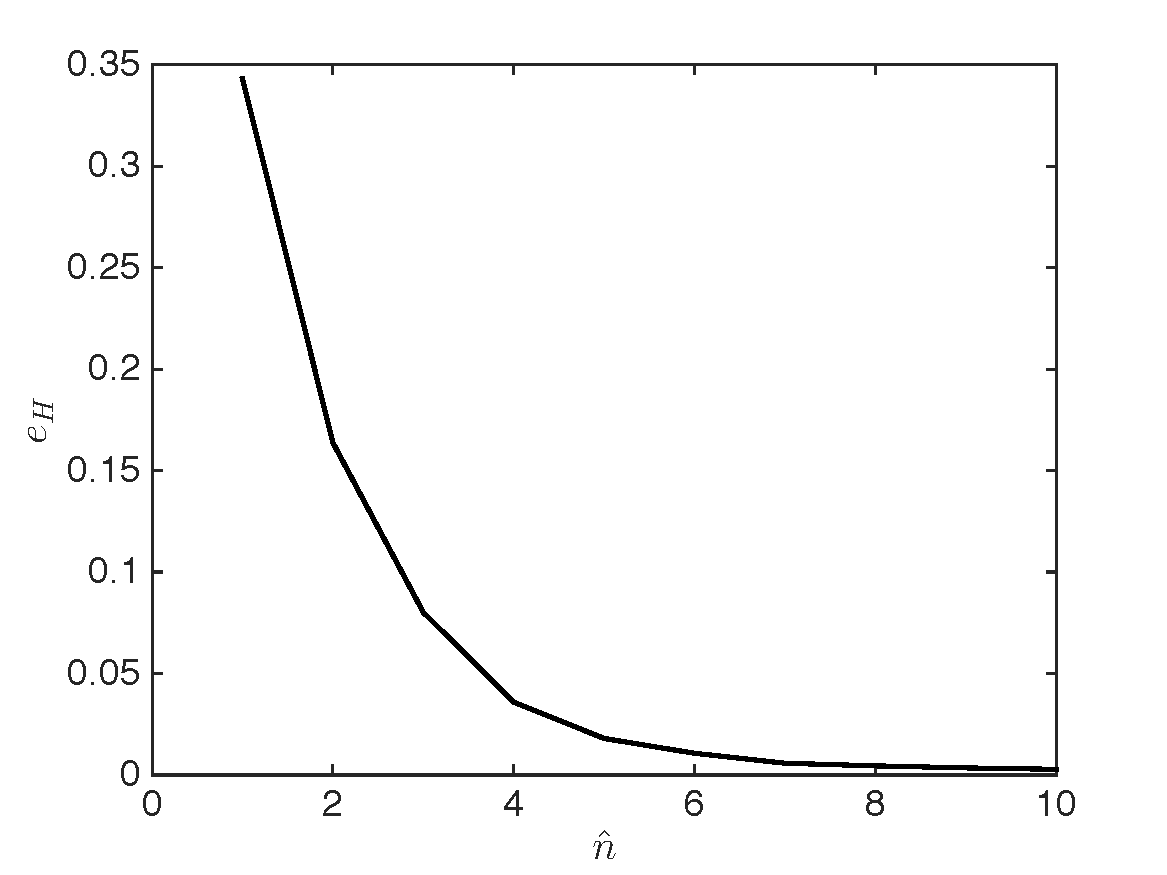
\includegraphics[width=\textwidth]{JustifyApprox_eH.pdf}
        		\caption{Entropy Error}
        		\label{fig:H_err}
    	\end{subfigure}
	\begin{subfigure}[b]{0.45\textwidth}
        		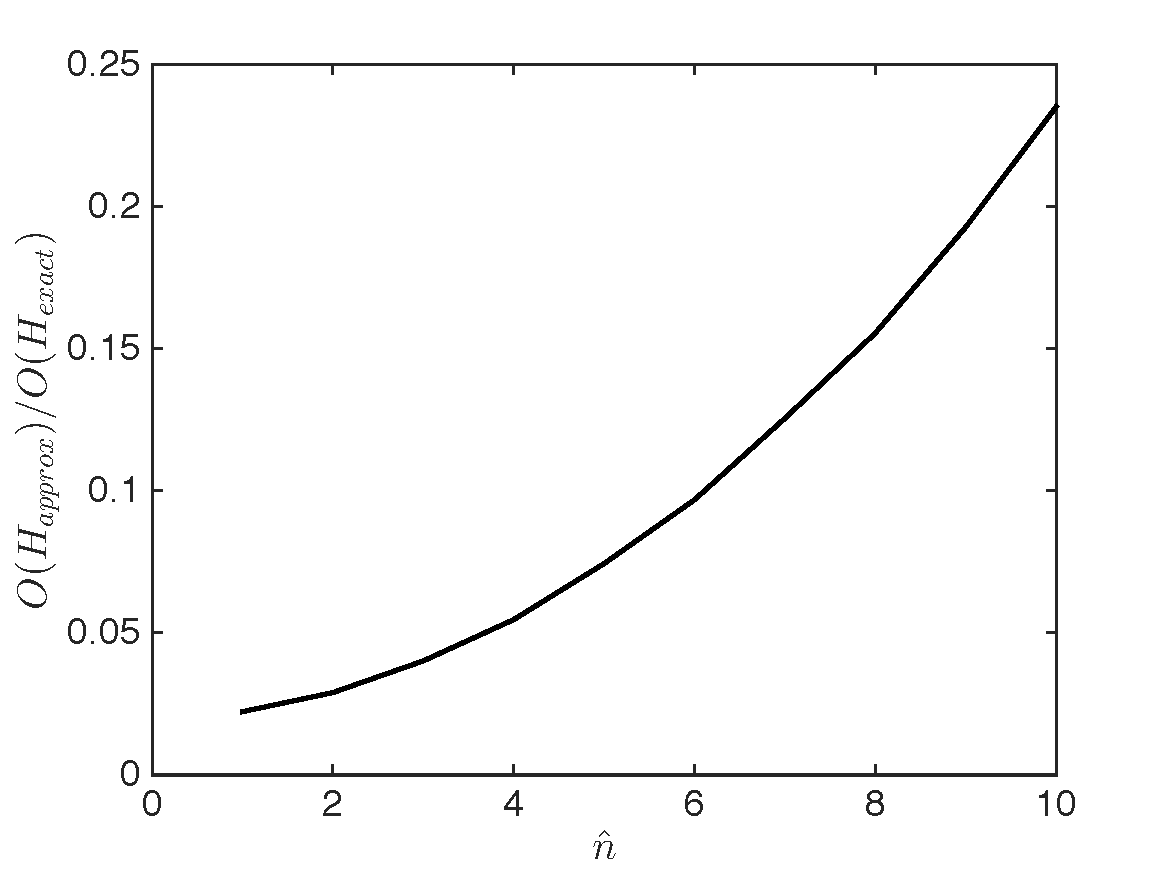
\includegraphics[width=\textwidth]{JustifyApprox_t.pdf}
        		\caption{Computation Ratio}
        		\label{fig:H_comp_ratio}
    	\end{subfigure}
	\caption{Expected Entropy Computational Improvement of Reduced Ray Cells Considered}
	\medskip
	\small
	The entropy error is decreased at the cost of increasing computation time in this Monte Carlo 1D measurement ray expected entropy case.
	\label{fig:ApproxJust}
\end{figure}





\section{Future Pose Optimization}

In this section, we show how expected entropy changes from single measurement rays can be integrated into predicting the expected information gain of measurement scans. This metric, and a cost associated with travel time, are combined to determine an optimal future pose and collision-free path in a 2D environment.

\subsection{Optimal Pose from Sample Rays}
\label{sec:OptimalPose2DMap}

The objective is to choose a future pose that minimizes the map uncertainty, such that the robot can autonomously move toward this optimal goal. The robot pose is selected among various positions and attitudes. Since searching over all locations and attitudes would require infinite computational resources, these search spaces are discretized into a limited number of robot attitudes and positions.
The procedure involves three steps. First, the attitude that maximizes the information gain objective function is selected at each candidate future pose location. Second, the location with the maximum objective function of all candidates is selected. Thus, the optimal attitude and the optimal location compose the optimal future pose. Finally, the robot determines and follows a collision-free path to the optimal future pose. This process is repeated, resulting in autonomous exploration.

\paragraph{Attitude Optimization}
Consider a collision-free pose candidate at an arbitrary location $x_c$. At this pose, consider $n_d$ evenly-spaced measurement rays oriented radially outward from the robot in a circular pattern (see red lines in Figure \ref{fig:OptProcess}). These rays are denoted $\braces{z_{c,1},z_{c,2},\ldots,z_{c,n_d}}$. Attitudes correspond to the rays such that the robot sensor is aligned with the ray direction, and these are denoted $\braces{R_{c,1},R_{c,2},\ldots,R_{c,n_d}}$, where the scan with attitude $R_{c,d}$ might cover several ray directions depending on the sensor FOV. We choose optimal attitude $R_c^*$ as the summation of the expected entropy changes covered by the scan,
\begin{align}
\label{eqn:FindRc}
&R_c^*=\argmax_{R_{c,d}}\sum_{z_{c,i}\in R_{c,d}\text{ FOV}}\bigg(H(P(m))
-\text{E}[H(P(m|x_c,z_{c,i}))]\bigg).
%\mathcal I_\text{ray}(x_c,z_{c,i})\right).
\end{align}

This method provides the attitude that maximizes the information gain at an arbitrary location in 2D space. The set of candidate positions that warrant consideration is determined with one of two methods, namely \emph{expanding ring} and \emph{complete Cartesian}, described next.

\paragraph{Expanding Ring}
The expanding ring technique is advantageous for searching local solutions quickly, only considering distant future poses when necessary. The key idea is that future candidate locations lie on a circular ``ring'' centered around the robot, evenly spaced around the ring (see red circles in Figure \ref{fig:OptProcess}), and the ring is expanded if certain criteria are not met. More explicitly, consider $n_c$ candidate locations denoted by $x_c\in\braces{x_1,x_2,\ldots,x_{n_c}}$ located with the distance $\delta$ away from the robot. All candidates must satisfy the inequality constraint,
\begin{align}
\label{eqn:CollisionInequalityConstraint}
P_\text{collision}(X)=1-\prod_{i\in\mathcal C_X}(P(\bar{\mathbf{m}}_i)\leq\beta,
\end{align}
where $\mathcal C_X$ is the set of grid cells falling inside a volume of preselected size around $X$ that may cause collision and $\beta>0$ is a small acceptable probability of collision. Any location that violates an inequality constraint \refeqn{CollisionInequalityConstraint} is excluded to avoid collisions. The set of optimal attitudes at each candidate location is $\braces{R^*_{1},R^*_{2},\ldots,R^*_{n_c}}$, obtained from \refeqn{FindRc}. The information gain objective function for a scan $Z_c$ captured from pose $X_c$ is
\begin{align}
\label{eqn:ObjFun}
\mathcal I(X_c)=H(P(m))-\text{E}\left[H(P(m|X_c,Z_c))\right],
\end{align}
is computed by a summation about the $n_d$ rays as %\refeqn{Objective},
\begin{align}
\label{eqn:ObjFunApprox}
\mathcal I(x_c,R_c^*)&\approx \sum_{z_{c,i}\in R_{c}^*\text{ FOV}}\bigg(H(P(m))-\text{E}\left[H(P(m|x_c,z_{c,i}))\right]\bigg),
\\
x_c^*&=\argmax_{x_c}\mathcal I(x_c,R_c^*).
\end{align}
At the optimal pose $X^*_c=(x^*_c,R^*_c)$, the resulting information gain must satisfy $\mathcal I(X_c^*)\geq\mathcal I_\text{min}$, where $\mathcal I_\text{min}$ is a minimum threshold for expected information gain; robot motion is only justified when the expected information gain is significantly large. If the minimum threshold is not met, the ring of candidate pose locations is increased such that $n_c$ and $\delta$ are multiplied by a scale function $\lambda>1$.
This process is repeated until the expected information gain of the optimal pose is at least $\mathcal I_\text{min}$, or all candidates lie in collision zones or outside map limits. %A pseudo-code of the process is found in Table \ref{tab:Alg_AutomousExploration}.

The primary advantage of the expanding ring approach to search the 2D space is that the number of pose candidates need not be proportional to the map area, and that local maxima tend to fall within short distances of the current robot pose. Additionally, the distance to these poses need not be explicitly considered in the pose determination optimization because the distance costs are identical to each candidate, assuming objects do not occlude the trajectories. The main drawback is that poses outside a small local region of the robot are frequently neglected, causing the robot to repeatedly execute short motions, often without large information gains.

\paragraph{Complete Cartesian}
The complete Cartesian method to search the 2D space provides candidates located fixed distance $d$ apart in each Cartesian direction. This approach is advantageous for capturing expected information gains in regions outside of the immediate vicinity of the robot, but must be applied carefully to avoid issues with computational bottlenecks due to the potentially-large search space.

Similar to the expanding ring approach, $n_c$ candidate pose locations are considered, where those violating \refeqn{CollisionInequalityConstraint} are neglected from further consideration. However, unlike the ring expanding approach, the candidates have different distances from the robot in general, so the objective function is modified to enforce a cost on the squared distance from the current pose location $x_t$ to the candidate location $x_c$, i.e.,
\begin{align}
\label{eqn:ObjFunApproxCompleteCartesian}
\mathcal I(x_c,R_c^*,x_t)\approx \sum_{z_{c,i}\in R_{c}^*\text{ FOV}}\bigg(H(P(m))-\text{E}\left[H(P(m|x_c,z_{c,i}))\right]\bigg)-k_\text{dist}\norm{x_t-x_c}^2,
\end{align}
where weighting function $k_\text{dist}$ represents the sensitivity to avoiding large motions across the map. Furthermore, the same candidate locations are considered throughout the repeated processes of exploration, and the map cell occupancies are assumed static. Therefore, if candidate location $x_c$ fails to satisfy $\mathcal I(x_c,R_c^*,x_t)+k_\text{dist}\norm{x_t-x_c}^2\geq\mathcal I_\text{min}$, then $x_c$ need \emph{never} be considered again. Avoiding these unnecessary calculations yields a greatly lowered computational burden, particularly late in exploration where several regions are collision-free but disadvantageous to revisit.


\begin{figure}
\vspace*{0.1\columnwidth}
\centerline{
	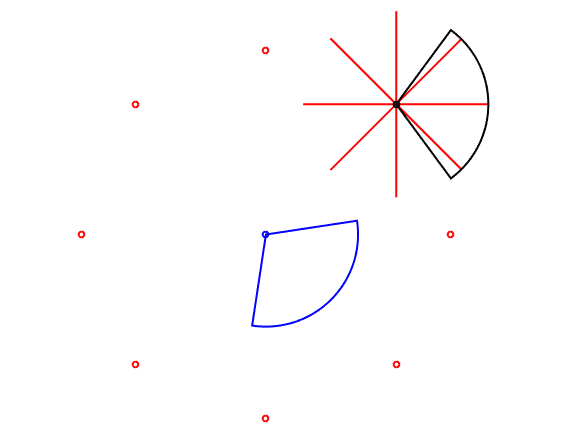
\includegraphics[height=0.35\columnwidth]{ExampleOptimalPose.png}
}
\begin{picture}(0,0)(0,0)
\setlength{\unitlength}{0.1\columnwidth}\scriptsize
\put(4.4,2.1){\color{blue}$X_t$}
\put(5.9,1.9){\color{red}$x_1$}
\put(2.9,2.0){\color{red}$x_5$}
\put(4.4,3.6){\color{red}$x_3$}
\put(4.4,0.6){\color{red}$x_7$}
\put(5.4,3.0){\color{red}$x_2$}
\put(3.3,3.1){\color{red}$x_4$}
\put(3.3,1.0){\color{red}$x_6$}
\put(5.4,1.0){\color{red}$x_8$}
\put(6.8,3.1){\color{red}$z_{2,1}$}
\put(4.5,3.1){\color{red}$z_{2,5}$}
\put(5.6,4.1){\color{red}$z_{2,3}$}
\put(5.6,2.2){\color{red}$z_{2,7}$}
\put(6.5,3.7){\color{red}$z_{2,2}$}
\put(4.9,3.8){\color{red}$z_{2,4}$}
\put(5.0,2.5){\color{red}$z_{2,6}$}
\put(6.5,2.5){\color{red}$z_{2,8}$}
\put(6.1,2.9){$X_c^*$}
\end{picture}
\caption{Optimal Pose Selection Illustration
}
\centering{
	\medskip
	\small
	This figure illustrates the expanding ring method. Initially, a robot (blue circle) views down and left (blue sector). Then, the robot considers $n_c=8$ poses (red circles) as possible candidates for where to move next. For each candidate, $n_d=8$ directions are considered (red lines, only displayed on candidate location $c=2$). Then, the expected entropy of each ray is calculated. The scan (red sector) covering those rays with the largest expected entropy decrease is chosen for each candidate, and the best candidate $X_c^*$ (black circle: location, black sector: scan) is chosen to maximize information gain. Finally, Dijkstra's algorithm provides the collision-free motion between $X_t$ and $X_c^*$, and the process is repeated.
}
\label{fig:OptProcess}
\end{figure}

% TODO: move these to 3D/multi-vehicle sections
%\subsection{Travel Cost with Obstacles}
% Dijkstra's cost map
%\subsection{Optimal Pose Selection}
% Single-Vehicle argmax

\subsection{Collision-Free Motion Planning}
% Dijkstra's algorithm (after cost map), no least squares yet

There are two important steps to moving a robot on a collision-free trajectory to its optimal pose. First, Dijkstra's algorithm~\cite{Dij59,Dij11} provides the cost map and optimal collision-free waypoints. Then, a constrained polynomial least squares trajectory serves as the desired path, which is followed by a controller.

\paragraph{Dijkstra's Search}

Dijkstra's search is naturally applied to this problem because the occupancy grid map serves nicely as a graph, and Dijkstra's algorithm provides an optimal collision-free trajectory along that graph. There are two steps to Dijkstra's algorithm: first, generate a cost map from the robot location to each grid cell on the 2D occupancy grid map. Only cells that satisfy \refeqn{CollisionInequalityConstraint} are considered to avoid possible collisions. Traveling to a neighboring cells that shares an edge costs the edge length distance $\alpha$, and the cost to travel to cells that share a corner is $\sqrt{2}\alpha$. This provides the collision-free distances to all reachable locations on the map. Second, the waypoints from a candidate pose to the current robot pose are easily obtained along the cost map using steepest descent. 


\paragraph{Constrained Polynomial Least Squares Trajectory} The trajectory to follow the path outlined by Dijkstra's algorithm is determined with a linear constrained least squares optimization, assuming the robot follows a polynomial trajectory with fixed speed. The starting and ending positions and attitudes may be constrained, and polynomials patched together for long trajectories share a common position and velocity with respect to time. Then, a controller on the robot tracks this trajectory until the robot falls within acceptable thresholds of the final optimal pose. Any control scheme for the motion of the robot can be integrated with the proposed exploration algorithm. Once the robot completes this motion, the entire process is repeated. 

\section{Numerical Examples}
\label{sec:Ae2DNumExamples}

Here we present two numerical examples. The first uses the expanding-ring technique in a small environment and the second considers a larger benchmark environment, so the complete Cartesian method is applied, as described in Section \ref{sec:OptimalPose2DMap}.

\subsection{Exploring a Simple Environment}
% SIMPAR numerical example (2 rooms, 1 hallway)

Here, a robot autonomously maps and explores a 2D environment composed of two rooms and one hallway. The robot models its surroundings with an occupancy grid of $15,000$ cells where grid cell edges have length $\alpha=0.2$m, composing a map with dimensions $30\text{m}\times20\text{m}$. The initial probability $P(\mathbf{m}_i)=1\times10^{-10}\approx0$ (minimum value for free space) for grid cells covered by the circular robot of radius $0.1$m and $P(\mathbf{m}_i)=0.5$ for all other cells.
At each time step, the robot receives a measurement scan, where the probabilistic properties of the sensor are taken from~\cite{PirRutBisSch11,KhoElb12}. Then, the $n_c=8$ evenly-spaced candidate locations about a circle of radius $\delta=0.5$m around the current pose location are considered, where $n_d=32$ measurement rays are evenly-spaced about the candidate location.  When no current candidates yield expected information gains above $\mathcal I_\text{min}=2$, $\lambda=1.25$ is multiplied to $n_c$ and $\delta$. The motion of the robot is restricted to movement along cells satisfying \refeqn{CollisionInequalityConstraint} with $\beta=0.01$. Dijkstra's algorithm provides collision-free motion planning.
The results are illustrated in Figure \ref{fig:AutonomousExploration}.


\begin{figure}
\centering{
    	\begin{subfigure}[b]{0.3\textwidth}
        		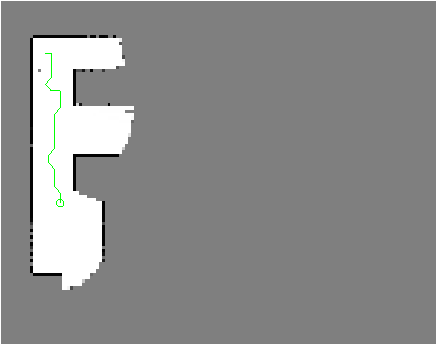
\includegraphics[width=\textwidth]{CDC16_t50.png}
        		\caption{Map at $t=50$ sec}
%        		\label{fig:}
    	\end{subfigure}
	\hspace*{0.01\columnwidth}
	\begin{subfigure}[b]{0.3\textwidth}
        		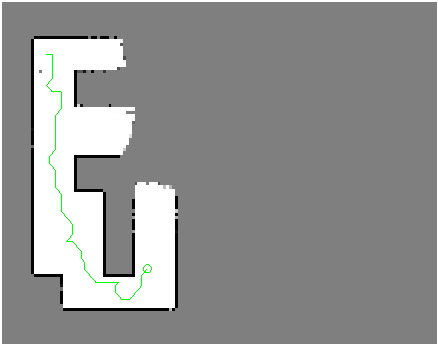
\includegraphics[width=\textwidth]{CDC16_t100.png}
        		\caption{Map at $t=100$ sec}
%        		\label{fig:}
    	\end{subfigure}
	\hspace*{0.01\columnwidth}
	\begin{subfigure}[b]{0.3\textwidth}
        		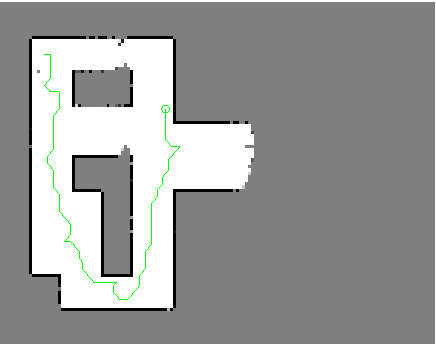
\includegraphics[width=\textwidth]{CDC16_t150.png}
        		\caption{Map at $t=150$ sec}
%        		\label{fig:}
    	\end{subfigure}
}
\centering{
    	\begin{subfigure}[b]{0.3\textwidth}
        		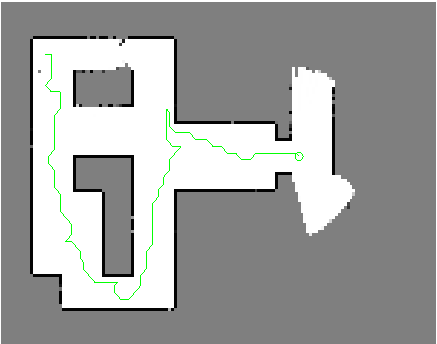
\includegraphics[width=\textwidth]{CDC16_t200.png}
        		\caption{Map at $t=100$ sec}
%        		\label{fig:}
    	\end{subfigure}
	\hspace*{0.01\columnwidth}
	\begin{subfigure}[b]{0.3\textwidth}
        		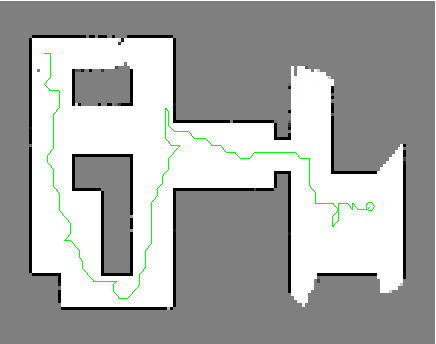
\includegraphics[width=\textwidth]{CDC16_t250.png}
        		\caption{Map at $t=250$ sec}
%        		\label{fig:}
    	\end{subfigure}
	\hspace*{0.01\columnwidth}
	\begin{subfigure}[b]{0.3\textwidth}
        		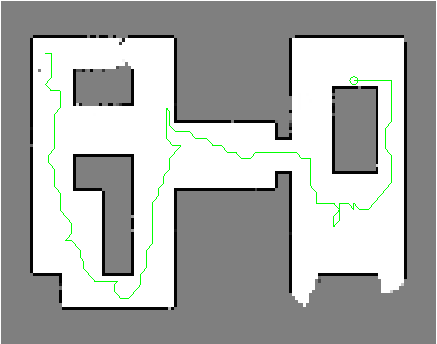
\includegraphics[width=\textwidth]{CDC16_t300.png}
        		\caption{Map at $t=300$ sec}
%        		\label{fig:}
    	\end{subfigure}
}
\centering{
    	\begin{subfigure}[b]{0.3\textwidth}
        		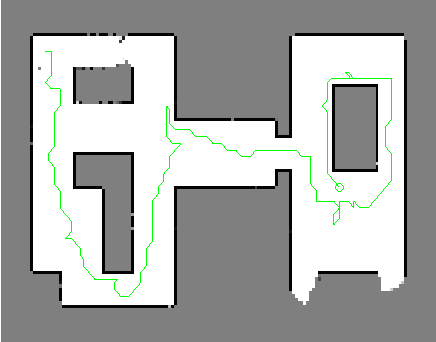
\includegraphics[width=\textwidth]{CDC16_t350.png}
        		\caption{Map at $t=350$ sec}
%        		\label{fig:}
    	\end{subfigure}
	\hspace*{0.01\columnwidth}
	\begin{subfigure}[b]{0.3\textwidth}
        		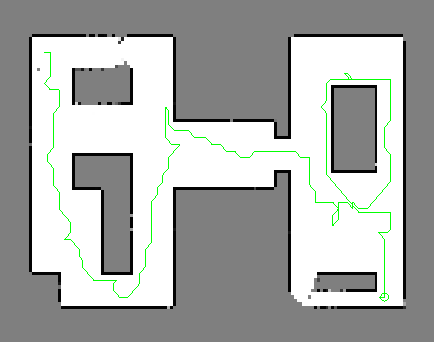
\includegraphics[width=\textwidth]{CDC16_t400.png}
        		\caption{Map at $t=400$ sec}
%        		\label{fig:}
    	\end{subfigure}
	\hspace*{0.01\columnwidth}
	\begin{subfigure}[b]{0.3\textwidth}
        		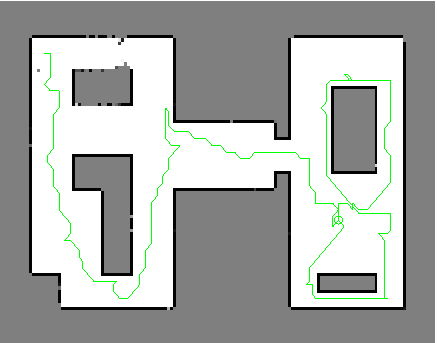
\includegraphics[width=\textwidth]{CDC16_t450.png}
        		\caption{Map at $t=450$ sec}
%        		\label{fig:}
    	\end{subfigure}
}
	\caption{Autonomous Exploration of a 2D Space Using the Expanding Ring Approach}
	\medskip
	\small
	A robot (green circle, green marker of previous path) measures a room with a Kinect depth sensor to maximize map information gain.
\label{fig:AutonomousExploration}
\end{figure}

Knowing only that the robot is inside free space at the beginning, the robot carefully navigates the environment while avoiding collisions. The robot motion is governed by a policy that maximizes the map information gain within its set of pose candidates, where the $\hat n=6$ is chosen to approximate the expected entropy of each ray. 
When running the exploration algorithm within the framework of the Robot Operating System (ROS)~\cite{ROS}, the mean computation time is $0.0194$ seconds to determine the optimal future pose and complete Dijkstra's algorithm on the occupancy grid.
The computation times for this map reached roughly $1$ second at maximum, corresponding to rare cases when the robot is locally surrounded by a highly-certain environment; this task requires evaluating many more pose candidates and motion planning over a larger terrain.

Throughout the numerical example, the robot chooses numerous actions, based directly on their expected information gains, not frontiers or predicted measurement scans. If the obstacles were known a priori, the motion planning problem would yield a simpler path; however, the autonomous exploration is based on only the information of the map that the robot generates, so the motion planning must be reevaluated repeatedly. Even with these limitations, the robot explores the vast majority of reachable space in the $450$ second period. 





\subsection{Exploring a Complicated Benchmark Environment}

Next, the proposed autonomous exploration approach is applied to the floor plan of the Intel Research Lab, illustrated in Figure~\ref{fig:intel}.
The robot explores its surroundings with an occupancy grid with $90,000$ cells where grid cell edges are $\alpha=0.1$m, composing a map with dimensions $30\text{m}\times30\text{m}$.
Similar to the prior example, the initial probability $P(\mathbf{m}_i)=1\times10^{-10}\approx0$ (minimum value for free space) is chosen for grid cells covered by the circular robot of radius of $0.3$m and $P(\mathbf{m}_i)=0.5$ for all other cells.
For added safety, cells falling within $0.6$m of the robot are considered inside the possible collision zone $\mathcal{C}_X$, from \refeqn{CollisionInequalityConstraint}, where $\beta=0.1$ is selected. 

The robot follows the complete Cartesian candidate search method to determine future poses, with $k_\text{dist}=5$ to avoid large motions with little added expected information gains. Due to the large size of the map, candidates below the expected information gain of $1.25$ are neglected from future consideration.

The time sequence of the exploration for every 5~minutes are simulated in the ROS Stage 2D environment. The corresponding simulation results are illustrated in Figure \ref{fig:IRL} and a video is available at \href{https://www.youtube.com/watch?v=5VdzKHreB_s}{\WriteBlue{https://www.youtube.com/watch?v=5VdzKHreB\_s}}.
Lighter red dots and darker blue dots in the explored area correlate to the level of information gain at those positions with low and high value, respectively. It is shown that the proposed autonomous exploration algorithm successfully mapped the complicated environment composed of a number of rooms, narrow hallways, and open spaces that are irregularly shaped.


\begin{figure}
	\centering
	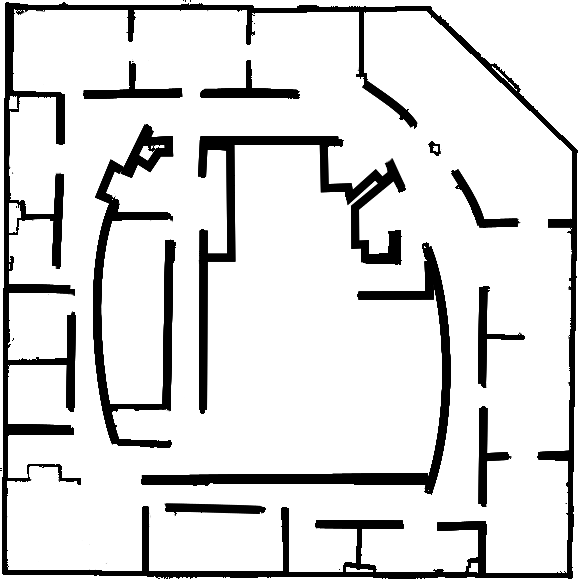
\includegraphics[width=0.4\textwidth]{intel_clean.png}
	\caption{Intel Research Lab Floor Plan Benchmark}
	\medskip
	\small
	The 2D floor plan from the Intel Research Lab~\cite{kummerle2009measuring} is simplified to eliminate small objects. The remaining black pixels are used to produce walls for 2D simulations.
\label{fig:intel}
\end{figure}


\begin{figure}[!ht]
    \centering
    \begin{subfigure}[t]{0.3\columnwidth}
        \centering
        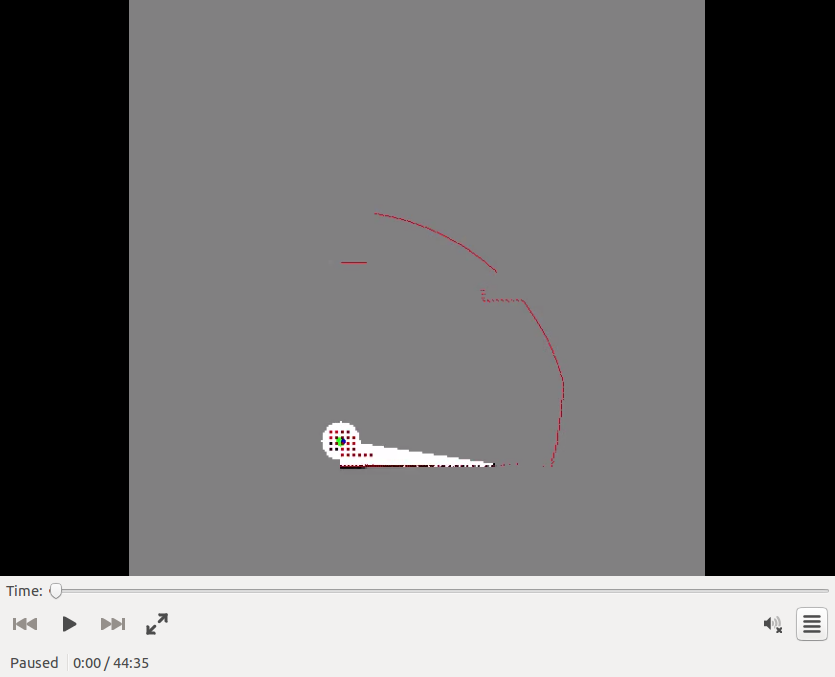
\includegraphics[trim = {4.6cm 3.8cm 4.6cm 0}, clip, width=\textwidth]{0min.png}
        \caption{$t=0$ min}
        \label{fig:IRL0min}
    \end{subfigure}
    \begin{subfigure}[t]{0.3\columnwidth}
        \centering
        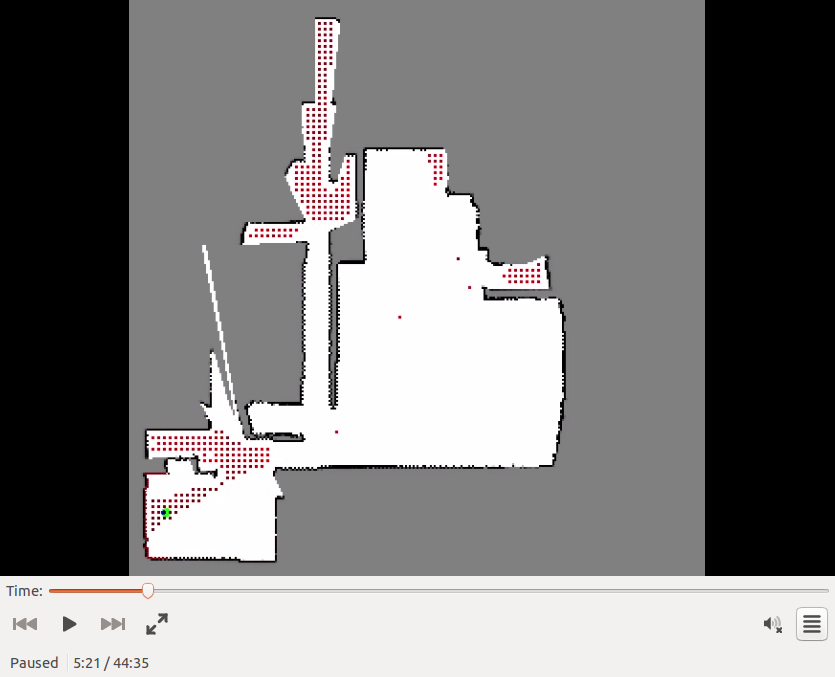
\includegraphics[trim = {4.6cm 3.8cm 4.6cm 0}, clip, width=\textwidth]{5min.png}
        \caption{$t=5$ min}
        \label{fig:IRL5min}
    \end{subfigure}
    \begin{subfigure}[t]{0.3\columnwidth}
           \centering
           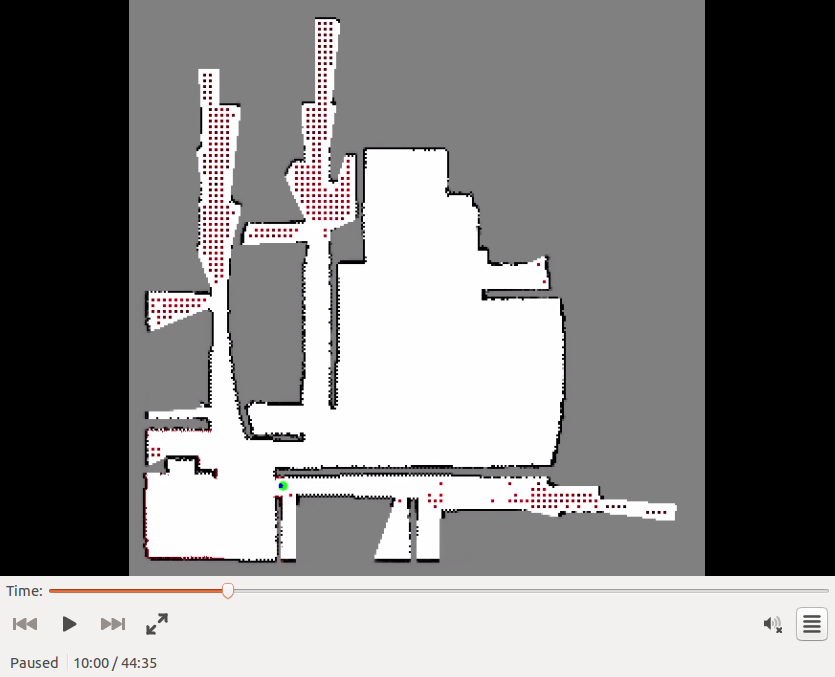
\includegraphics[trim = {4.6cm 3.8cm 4.6cm 0}, clip, width=\textwidth]{10min.png}
        \caption{$t=10$ min}
        \label{fig:IRL10min}
    \end{subfigure}
    \begin{subfigure}[t]{0.3\columnwidth}
           \centering
           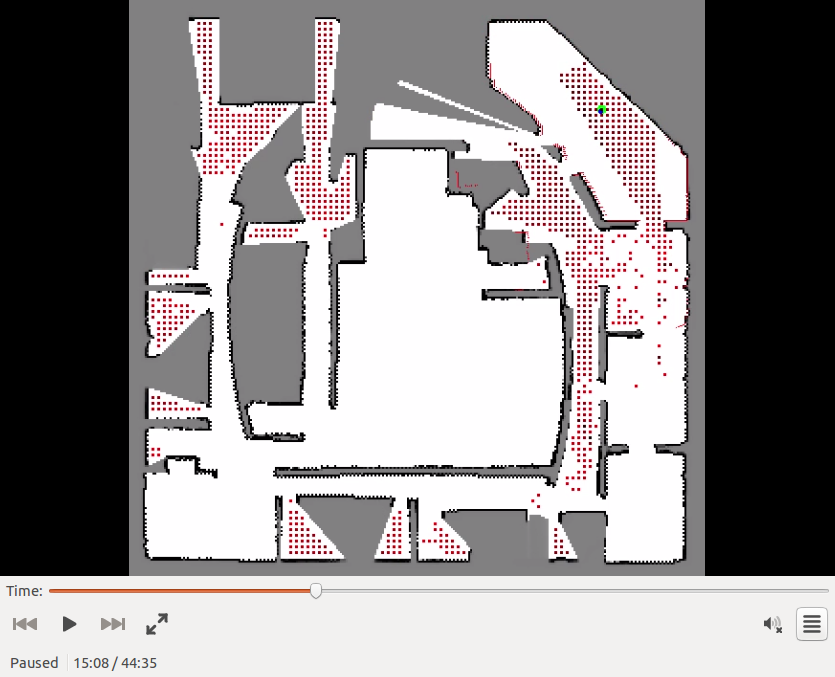
\includegraphics[trim = {4.6cm 3.8cm 4.6cm 0}, clip, width=\textwidth]{15min.png}
        \caption{$t=15$ min}
        \label{fig:IRL15min}
    \end{subfigure}
    \begin{subfigure}[t]{0.3\columnwidth}
         \centering
         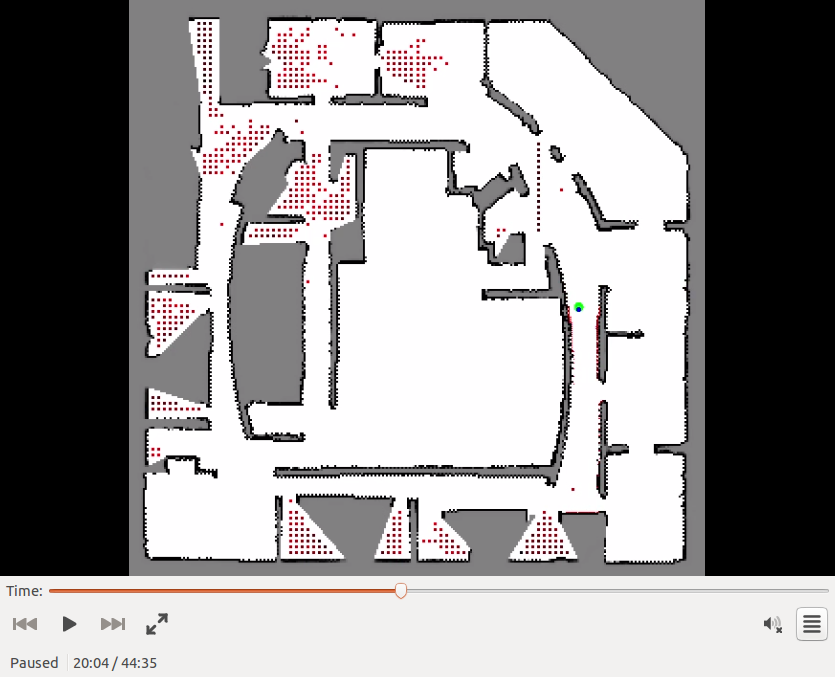
\includegraphics[trim = {4.6cm 3.8cm 4.6cm 0}, clip, width=\textwidth]{20min.png}
        \caption{$t=20$ min}
        \label{fig:IRL20min}
    \end{subfigure}
    \begin{subfigure}[t]{0.3\columnwidth}
           \centering
           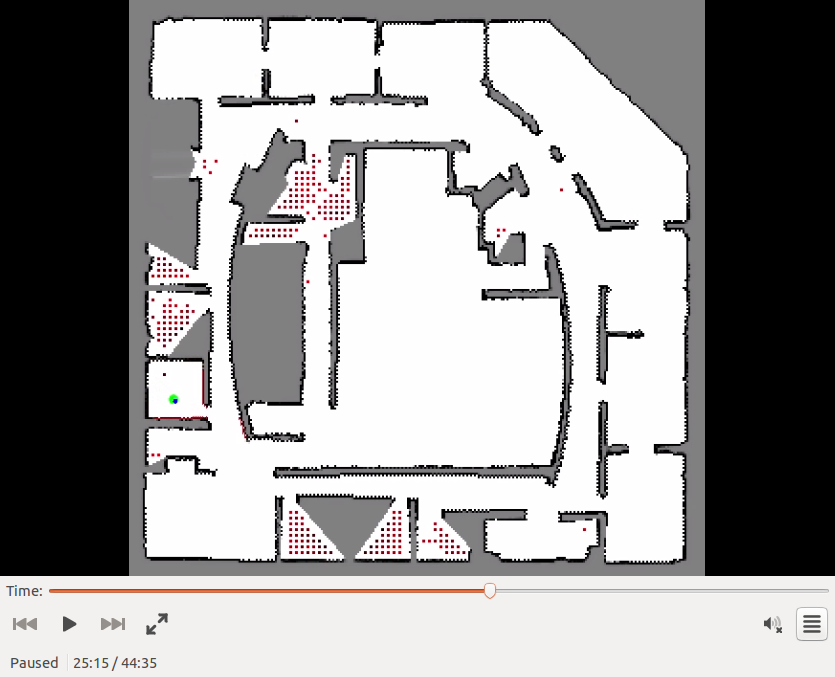
\includegraphics[trim = {4.6cm 3.8cm 4.6cm 0}, clip, width=\textwidth]{25min.png}
        \caption{$t=25$ min}
        \label{fig:IRL25min}
    \end{subfigure}
    \begin{subfigure}[t]{0.3\columnwidth}
           \centering
           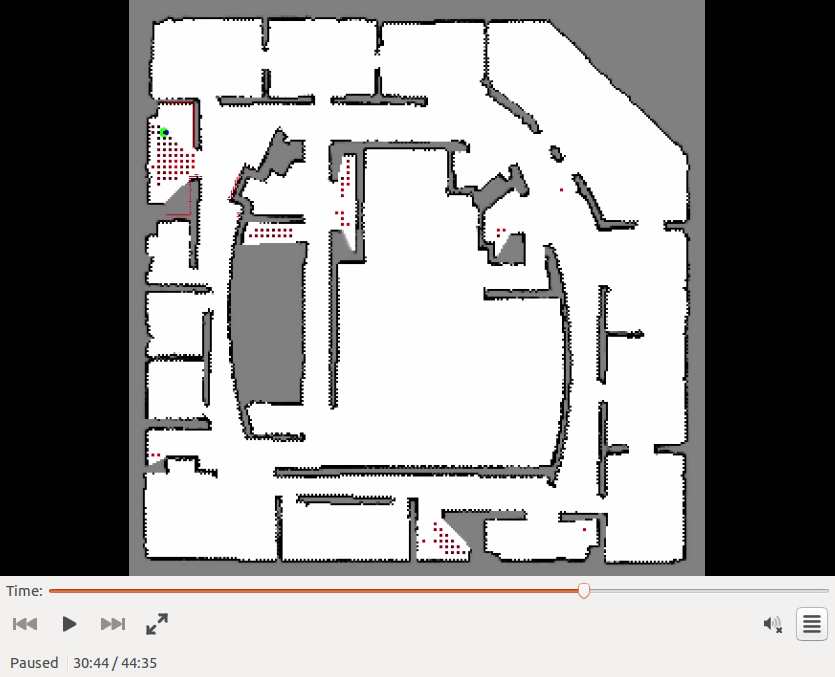
\includegraphics[trim = {4.6cm 3.8cm 4.6cm 0}, clip, width=\textwidth]{30min.png}
        \caption{$t=30$ min}
        \label{fig:IRL30min}
    \end{subfigure}
    \begin{subfigure}[t]{0.3\columnwidth}
           \centering
           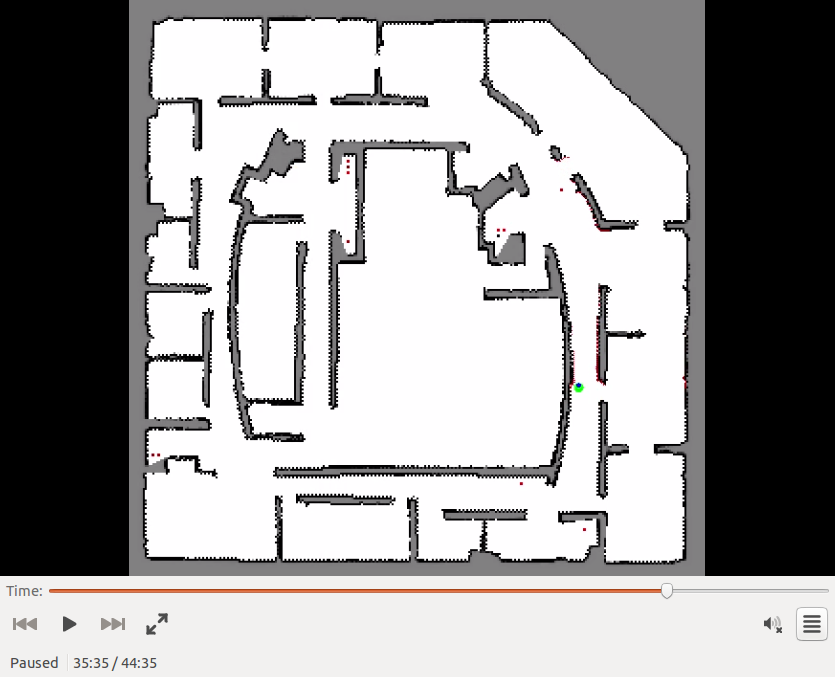
\includegraphics[trim = {4.6cm 3.8cm 4.6cm 0}, clip, width=\textwidth]{35min.png}
        \caption{$t=35$ min}
        \label{fig:IRL35min}
    \end{subfigure}
    \begin{subfigure}[t]{0.3\columnwidth}
           \centering
           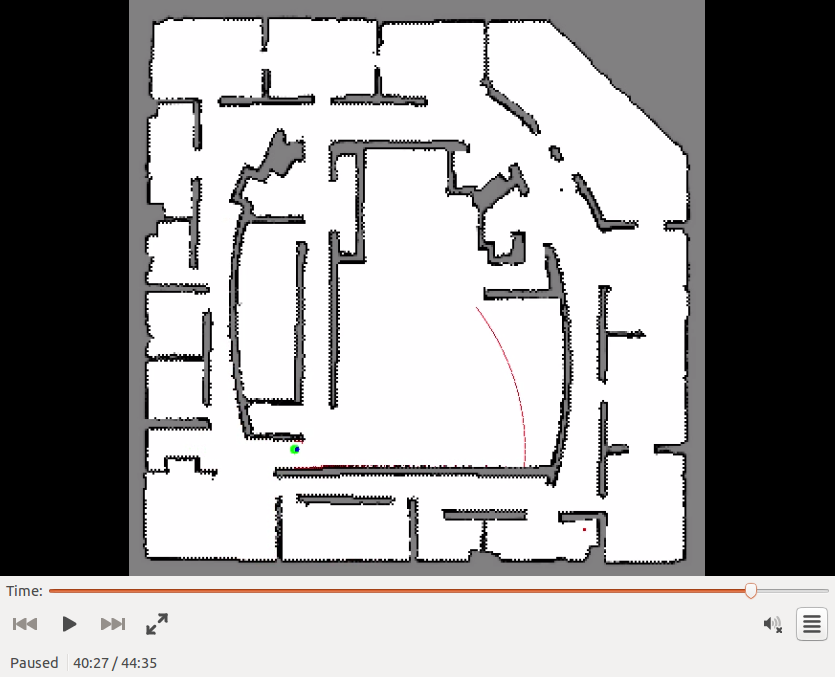
\includegraphics[trim = {4.6cm 3.8cm 4.6cm 0}, clip, width=\textwidth]{40min.png}
        \caption{$t=40$ min}
        \label{fig:IRL40min}
    \end{subfigure}
	\caption{Autonomous Exploration of the Intel Research Lab Using the Complete Cartesian Approach}
	\medskip
	\small
	A robot (green) measures a room in the ROS Stage simulator using the Intel Research Lab floor plan. The exact inverse sensor model is used for the autonomous exploration algorithm.
    \label{fig:IRL}
\end{figure}



% TODO: move these to final chapter
%\section{Experimental Result}
% JINT17 9, 10, 11 (ground experiment at the NRL)

\section{Conclusions}

The proposed autonomous exploration scheme determines the expected value of entropy for various potential robotic actions. The optimal policy maximizes an objective function that includes expected information gain and travel distance. Collision-free paths to optimal poses are determined with Dijkstra's search and a constrained polynomial least squares trajectory. These are demonstrated with two numerical examples, showing the expanding ring and complete Cartesian approaches. Due to superior scalability, the complete Cartesian approach is applied to subsequent exploration algorithms in this dissertation.
